%%%%%%%%%%%%%%%%%%%%%%%%%%%%%%%%%%%%%%%%%
% Beamer Presentation
% LaTeX Template
% Version 1.0 (10/11/12)
%
% This template has been downloaded from:
% http://www.LaTeXTemplates.com
%
% License:
% CC BY-NC-SA 3.0 (http://creativecommons.org/licenses/by-nc-sa/3.0/)
%
%%%%%%%%%%%%%%%%%%%%%%%%%%%%%%%%%%%%%%%%%

%----------------------------------------------------------------------------------------
%	PACKAGES AND THEMES
%----------------------------------------------------------------------------------------

\documentclass[xcolor={usenames,dvipsnames}]{beamer}
\usepackage{ctex}
\usepackage{beamerthemesplit} 
\mode<presentation> {

% The Beamer class comes with a number of default slide themes
% which change the colors and layouts of slides. Below this is a list
% of all the themes, uncomment each in turn to see what they look like.

%\usetheme{default}
%\usetheme{AnnArbor}
%\usetheme{Antibes}
%\usetheme{Bergen}
%\usetheme{Berkeley}
%\usetheme{Berlin}
%\usetheme{Boadilla}
%\usetheme{CambridgeUS}
%\usetheme{Copenhagen}
%\usetheme{Darmstadt}
%\usetheme{Dresden}
%\usetheme{Frankfurt}
%\usetheme{Goettingen}
%\usetheme{Hannover}
%\usetheme{Ilmenau}
%\usetheme{JuanLesPins}
%\usetheme{Luebeck}
\usetheme{Madrid}
%\usetheme{Malmoe}
%\usetheme{Marburg}
%\usetheme{Montpellier}
%\usetheme{PaloAlto}
%\usetheme{Pittsburgh}
%\usetheme{Rochester}
%\usetheme{Singapore}
%\usetheme{Szeged}
%\usetheme{Warsaw}

% As well as themes, the Beamer class has a number of color themes
% for any slide theme. Uncomment each of these in turn to see how it
% changes the colors of your current slide theme.

%\usecolortheme{albatross}
%\usecolortheme{beaver}
%\usecolortheme{beetle}
%\usecolortheme{crane}
%\usecolortheme{dolphin}
%\usecolortheme{dove}
%\usecolortheme{fly}
%\usecolortheme{lily}
%\usecolortheme{orchid}
%\usecolortheme{rose}
%\usecolortheme{seagull}
%\usecolortheme{seahorse}
%\usecolortheme{whale}
%\usecolortheme{wolverine}

%\setbeamertemplate{footline} % To remove the footer line in all slides uncomment this line
%\setbeamertemplate{footline}[page number] % To replace the footer line in all slides with a simple slide count uncomment this line

%\setbeamertemplate{navigation symbols}{} % To remove the navigation symbols from the bottom of all slides uncomment this line
}


\usepackage{graphicx} % Allows including images
\usepackage{booktabs} % Allows the use of \toprule, \midrule and \bottomrule in tables
\bibliographystyle{ieeetr}
\setbeamertemplate{footline}{%
	\leavevmode%
	\hbox{%
		\begin{beamercolorbox}[wd=.45\paperwidth,ht=2.25ex,dp=1ex,center]{author in head/foot}%
			\usebeamerfont{section in head/foot}\insertsectionnavigationhorizontal{.45\textwidth}{}{}
		\end{beamercolorbox}%
		\begin{beamercolorbox}[wd=.22\paperwidth,ht=2.25ex,dp=1ex,center]{title in head/foot}%
			\usebeamerfont{title in head/foot}\insertshorttitle
		\end{beamercolorbox}%
		\begin{beamercolorbox}[wd=.3333\paperwidth,ht=2.25ex,dp=1ex,right]{date in head/foot}%
			\usebeamerfont{date in head/foot}\insertshortdate{}\hspace*{2em}
			\insertframenumber{} / \inserttotalframenumber\hspace*{2ex}
		\end{beamercolorbox}}%
		\vskip0pt%
	}
%----------------------------------------------------------------------------------------
%	TITLE PAGE
%----------------------------------------------------------------------------------------

\title[课程设计]{\textbf{数据库/网络安全方向课程设计大作业答辩}} % The short title appears at the bottom of every slide, the full title is only on the title page

\author{邢元勋 \and 李欣宜} % Your name
\institute[DLUT] % Your institution as it will appear on the bottom of every slide, may be shorthand to save space
{
大连理工大学软件学院 \\ % Your institution for the title page
%\medskip
%\textit{john@smith.com} % Your email address
\url{https://github.com/Lixinyi-DUT/sctp_simulation}
}
\date{\today} % Date, can be changed to a custom date

\begin{document}

\begin{frame}
\titlepage % Print the title page as the first slide
\end{frame}
\section{概述}
\begin{frame}
\frametitle{\textbf{概览}} % Table of contents slide, comment this block out to remove it
\tableofcontents % Throughout your presentation, if you choose to use \section{} and \subsection{} commands, these will automatically be printed on this slide as an overview of your presentation
\end{frame}

%----------------------------------------------------------------------------------------
%	PRESENTATION SLIDES
%----------------------------------------------------------------------------------------
\begin{frame}
	\frametitle{\textbf{主要工作}}
	\begin{itemize}
		\item 了解~SCTP~协议工作机制
		\item 了解基于~SCTP~\textcolor{blue}{多宿主特性}的~CMT~传输机制
		\item 寻找~SCTP~在\textcolor{blue}{无线}网络中的应用
		\item 提出可能的改进方案
		\item 针对几种典型的~SCTP~有线网络结构进行模拟得到
		\begin{itemize}
			\item 丢包率
			\item 吞吐量
			\item 端到端时延
			\item 拥塞控制窗口大小
		\end{itemize}
		等参数,并进行分析
	\end{itemize}
\end{frame}
%------------------------------------------------
\section{背景} % Sections can be created in order to organize your presentation into discrete blocks, all sections and subsections are automatically printed in the table of contents as an overview of the talk
%------------------------------------------------

\subsection{SCTP协议简介}
\begin{frame}
	\frametitle{SCTP\textbf{协议}\cite{stewartstream}}
	\framesubtitle{\textbf{流传输控制协议}:\textbf{S}tream \textbf{C}ontrol \textbf{T}ransmission \textbf{P}rotocol}
	\begin{itemize}
		\item 与应用广泛的~\textcolor{RoyalPurple}{TCP}~、~\textcolor{PineGreen}{UDP}~协议相似,SCTP~作为一种\textcolor{blue}{传输层}协议在计算机网络中使用。
		\item 基于\textcolor{PineGreen}{基于不可靠传输业务的协议}之上的\textcolor{RoyalPurple}{可靠的数据报传输协议}
		\item \textcolor{PineGreen}{面向消息}(message-oriented):以消息(比特组)的形式传输数据,将数据和控制信息划分为组块(chunk)		
		\item 多流(multi-streaming): 并行传送多个独立的数据流
		\item 在一个数据流中,给每个消息指定序列号,以保证不同流的消息是\textcolor{RoyalPurple}{有序}的,也引入了\textcolor{RoyalPurple}{拥塞控制}
	\end{itemize}
\end{frame} 

\begin{frame}
	\frametitle{SCTP\textbf{协议特性}}
	\begin{itemize}
		\item 多宿主(multi-homing)支持:一个连接的端点可以拥有不止一个IP地址,缓解一条路径故障带来的威胁
		\item 消除了头阻塞(head-of-line blocking)
		\item 路径选择,主传输路径选择,测试传输路径的连通性
		\item 引入有效性和确认机制对抗洪泛攻击(四次握手),提供数据块重复和丢失通知	
		\item 使用SACK进行拥塞控制
	\end{itemize}
\end{frame}

\begin{frame}
	\frametitle{\textbf{多宿主支持}}
	\framesubtitle{\textbf{增加冗余IP地址,提高可达性}}
	\begin{block}{}
		节点使用心跳(heartbeat)检查对方的主地址和冗余地址的可达性,当收到heartbeat时需要确认回复ACK
	\end{block}
	\begin{alertblock}{}
			发送消息时,主IP由主机(而不是SCTP)决定
	\end{alertblock}
	\begin{figure}
		\includegraphics[width=0.7\linewidth]{pic/SCTP-multihoming.png}
		\caption{对称多宿主}
	\end{figure}
\end{frame}

\subsection{CMT}
\begin{frame}
	\frametitle{CMT:\textbf{并行多路传输}}
	\framesubtitle{\textbf{C}oncurrent \textbf{M}ultipath \textbf{T}ransfer}
	\begin{block}{\textbf{能被同时分配多个IP的主机是多宿主的}}
		利用SCTP的多宿主特性,使用多个端到端路径同时传送数据\cite{anardhan2012concurrent}
	\end{block}
	\begin{columns}
    \column{0.37\textwidth}
	\begin{picture}(150,50)(20,50)
	  \put(20,15) {主机A}
	  \put(120,15) {主机B}
	  \put(20,25) {\framebox(30,80){}}
	  \put(120,25) {\framebox(30,80){}}
	  \thicklines
	  {\color{red}{\put(50,90) {\vector(1,0){70}}}}
	  \put(50,40) {\vector(1,0){70}}
	  \put(50,75) {\vector(1,0){70}}
	  \put(75,55) {$\cdots$}
	  \put(21,92) {{\footnotesize 主IP($IP_0$)}}
	  \put(121,92) {{\footnotesize 主IP($IP_0$)}}
	  \put(32,40) {{\footnotesize $IP_n$}}
	  \put(121,40) {{\footnotesize $IP_n$}}
	  \put(32,75) {{\footnotesize $IP_1$}}
	  \put(121,75) {{\footnotesize $IP_1$}}	 
	  \put(34,55) {$\vdots$} 
	  \put(123,55) {$\vdots$} 
	  {\color{red}{\put(70,92) {{\footnotesize 主链路}}}}
	\end{picture}
	\column{0.55\textwidth}
	\begin{exampleblock}{}
		\begin{itemize}
			\item 用于提高吞吐量
			\item 瓶颈队列互相独立
			\item 使用SFR-CACC算法消除不必要的快速重传
			\item CUC算法解决拥塞窗口更新太少的问题
			\item DAC算法解决ack流量增加问题
		\end{itemize}
	\end{exampleblock}
	\end{columns}
\end{frame}
\subsection{无线SCTP}
\begin{frame}
	\frametitle{无线SCTP}
	\begin{alertblock}{mSCTP: Mobile SCTP}
		\begin{itemize}
			\item ADDIP扩展:满足动态建立连接要求,移动不再受到限制
			\item 移动节点和通信节点都支持动态地址配置扩展
		\end{itemize}
	\end{alertblock}
	
	\begin{block}{cSCTP: Celluar SCTP}
		在封包内引入变量handoff\_mode,切换效果更佳。
		\begin{description}
			\item[Layer3] Host-Agent:与接入路由(AR)通信
			\item[Layer4] cSCTP:SCTP增加动态地址设置扩展和切换流程
			\item[Layer5] 应用层SIP User Agent
		\end{description}	
    \end{block}
    	\begin{block}{\textbf{无线多跳网络}\cite{aydin2009performance}}
    		\begin{itemize}
    			\item IEEE 802.11(DCF)  CSMA/CA
    		\end{itemize}
    	\end{block}
\end{frame}


\section{优化方案}
\begin{frame}
	\frametitle{\textbf{优化方案}}
	\framesubtitle{\textbf{无线多跳网络环境下SCTP协议的吞吐量表现}}
	\begin{itemize}
		\item 采用OPNET模拟,通过改变接收方拥塞窗口的大小,源和目的地之间的跳数来分析实验结果,吞吐量随着跳数的增加而降低。
		\item 在跳数较少的情况下,需在博监听对吞吐量的增加帮助不大,丢包会导致SCTP超时,降低工作效率。
		\item 如果丢包的原因不是因为网络拥塞和SCTP窗口过小,就会很不公平。这种情况被称为“SMALL WINDOW SYNDROME”。
	\end{itemize}
	\begin{alertblock}{}
		解决该问题的办法是在传输的空闲阶段(idle period)传输丢失的数据报。
	\end{alertblock}
\end{frame}

\begin{frame}
	\frametitle{\textbf{优化方案}}
	\framesubtitle{\textbf{多路径并行传输中的吞吐量改进算法}}
	\begin{itemize}
		\item 多路径并行传输是一种有线情况下的传输过程,分为理想和非理想状态
		\item 理想状态下不考虑$throughput_r=ck_r/RTT_r$
		\begin{itemize}
			\item 即吞吐量等于$r$轮传输成功的数据包总和除以$r$轮中往返的时间的总和
		\end{itemize}
		\item 非理想状态下要考虑超时重传。
		\item 一般来说,一个路径发生故障时,会导致数据报传输失败,当重传次数超过检测阈值(PMR)时,路径会变为Failed状态。
	\end{itemize}
\end{frame}

\begin{frame}
	\frametitle{\textbf{优化方案}}
	\framesubtitle{\textbf{多路径并行传输中的吞吐量改进算法}}
	CMT-PF算法解决了上述问题:
	\begin{itemize}
		\item 当超时传输在传输路径上个产生时,则认为其进入PF(潜在失败)状态,并终止数据包的传输
		\item 进入PF状态的路径会发送HeartBeat包,若HB超过PMR值,则彻底进入Failed状态
		\item 否则路径仍为Active状态
	\end{itemize}
\end{frame}

\begin{frame}
	\frametitle{\textbf{优化方案}}
	\framesubtitle{SCTP\textbf{拥塞控制机制的研究与改进}}
	\begin{exampleblock}{SCTP vegas \textbf{算法}}
	  \begin{itemize}
			\item 以RTT的变化来判断网络拥塞的发生
			\item 由TCP vegas算法扩展而来
		\end{itemize}
	\end{exampleblock}
    发送端每收到一个数据报的ACK时,就会获得一个新的RTT样本,利用平均RTT作为判别标准,对RTT进行更新。

\end{frame}

\begin{frame}
	\frametitle{\textbf{优化方案}}
	\framesubtitle{SCTP\textbf{拥塞控制机制的研究与改进}}    \begin{exampleblock}{\textbf{慢启动方法的改进}}
		\begin{itemize}
			\item 当发送速率接近网络带宽时,逐渐减小拥塞窗口的增长速率,使其平滑的逼近网络带宽
			\item $cwnd < ssthreshold/2$ 时,与慢启动的原理一致
			\item $ cwnd > ssthreshold/2 $ 且 $ ssthreshold-cwnd > 1 $ 时,每个RTT内拥塞窗口增大
			\item $ ssthreshold-cwnd < 1 $ 时,进入拥塞避免
		\end{itemize}
	\end{exampleblock}
\end{frame}

\begin{frame}
	\frametitle{\textbf{优化方案}}
	\framesubtitle{SCTP\textbf{拥塞控制机制的研究与改进}}    
	\begin{equation*}
	cwnd(t+T)=
	\begin{cases}
	 2*cwnd(t) \qquad \qquad {\color{blue}{{\footnotesize \mbox{当} cwnd<ssthresh/2}}} \\
	 cwnd+Rtt(Rtt+MaxRtt)*(ssthresh-cwnd(t)) \\ 
	 {\color{blue}{{\footnotesize \mbox{当} cwnd \ge ssthresh/2 \mbox{且} ssthresh-cwnd>1}}} \\
	 ssthresh \qquad \qquad  {\color{blue}{{\footnotesize \mbox{其他}}}}
	\end{cases}
	\end{equation*}
\end{frame}
\section{实验}

\subsection{实验环境/工具}
\begin{frame}
	\frametitle{\textbf{实验环境/工具}}
	\begin{alertblock}{\textbf{实验环境}}
		\begin{itemize}
			\item Windows 8.1
			\item Cygwin \textcolor{gray}{(Easy 2007.3.21)}
			\item ns-2.34
		\end{itemize}
	\end{alertblock}
	\begin{block}{\textbf{实验工具}}
	\begin{description}
				\item[tcl/otcl] 脚本编写模拟测试
				\item [gawk] 读写/管理测试结果数据
				\item [R/ggplot2] 计算/分析/作图
	\end{description}
	\end{block}
\end{frame}

\begin{frame}
	\frametitle{\textbf{结果参数}}
	\begin{description}
		\item[丢包率] 丢失数据包占所发数据组的比率
		\item[吞吐量] 单位时间内,某个节点发送和接受的数据量
		\item[端到端时延] 数据包从离开源点时算起一直到抵达终点时一共经历了的时间,包括打包和解包的时延,和\textcolor{red}{网络传输时延}
		\item[cwnd] 拥塞窗口,大小取决于网络的拥塞程度,且动态变化
	\end{description}
\end{frame}

\subsection{实验过程}
\begin{frame}{\textbf{实验}1}
	\begin{columns}
		\column{0.45\textwidth}
		\begin{picture}(100,40)
		  \put(10,20){\circle{20}}
		  \put(90,20){\circle{20}}
		  \put(20,20){\line(1,0){60}}
		  \thicklines
		  {\color{red}{\put(25,25){\vector(1,0){50}}}}
		  \thinlines
		  \put(-2,0){{\footnotesize host\_0}}
		  \put(78,0){{\footnotesize host\_1}}
		\end{picture}
		\column{0.5\textwidth}
		\begin{tabular}{c|c}
			\hline
			参数 & 值 \\
			\hline
			传输层 & SCTP \\
			应用层 & FTP \\
			带宽 & 1Mb \\
		    时延 & 50ms \\
		    丢包率 & 0.01 \\
		    MTU & 1500 \\
		    数据组块大小 & 1468 \\
		    \hline
		\end{tabular}
	\end{columns}
\end{frame}

\begin{frame}
	\frametitle{\textbf{实验}1:\textbf{吞吐量}}
	\begin{figure}
		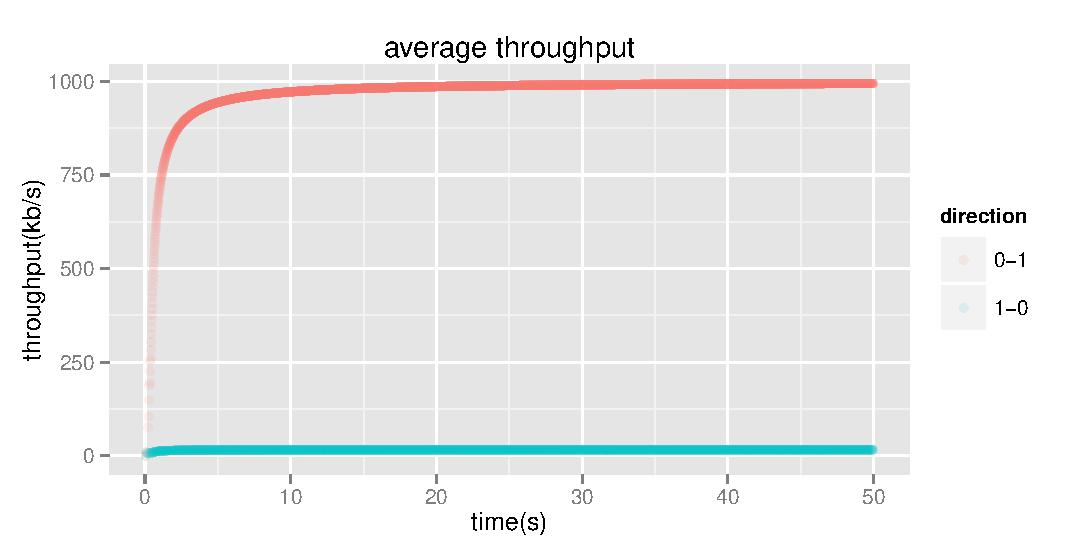
\includegraphics[width=\textwidth]{pic/plot_th_1.pdf}
	\end{figure}
\end{frame}

\begin{frame}
	\frametitle{\textbf{实验}1:\textbf{时延}}
	\begin{figure}
		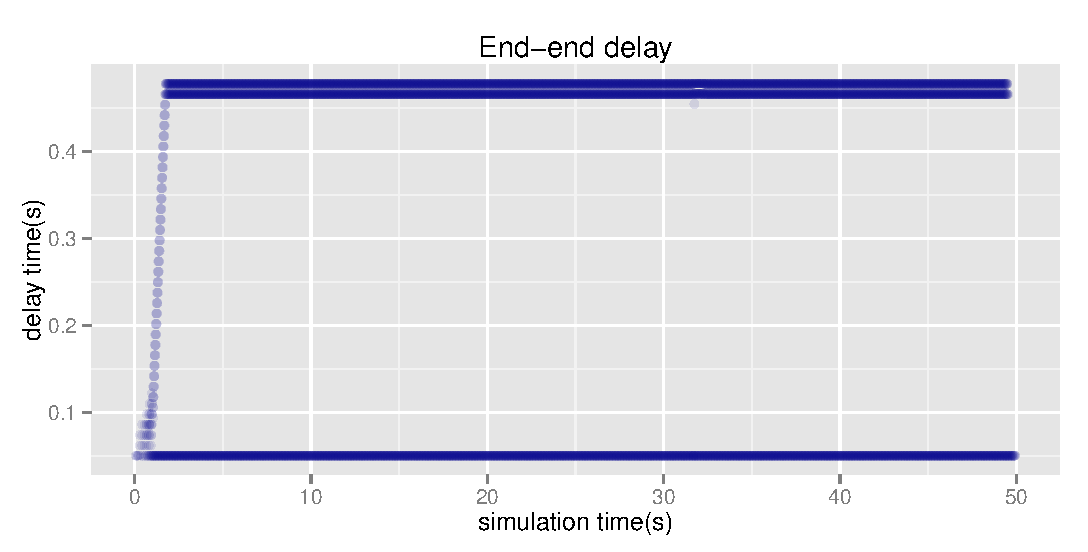
\includegraphics[width=\textwidth]{pic/plot_delay_1.pdf}
	\end{figure}
\end{frame}

\begin{frame}
	\frametitle{\textbf{实验}2}
	\framesubtitle{CMT\textbf{模拟},\textbf{使用}ReOrdering、CUC、AUC\textbf{算法},\textbf{引入}PF\textbf{机制}}
	\begin{columns}
		\column{0.45\textwidth}
		\begin{picture}(100,40)(-30,0)
		
		
		\put(10,20){\circle{20}}
		\put(90,20){\circle{20}}
		\put(10,10){\line(1,0){80}}
		\put(10,30){\line(1,0){80}}
		\thicklines
		{\color{red}{\put(25,5){\vector(1,0){50}}}}
		{\color{red}{\put(25,35){\vector(1,0){50}}}}
		\thinlines
		\put(-35,16){{\footnotesize host\_0}}
		\put(105,16){{\footnotesize host\_1}}
		\put(-2,0){{\footnotesize if\_1\textcolor{blue}{{\itshape{(2)}}}}}
		\put(80,0){{\footnotesize if\_1\textcolor{blue}{{\itshape{(5)}}}}}
		\put(-2,32){{\footnotesize if\_0\textcolor{blue}{{\itshape{(1)}}}}}
		\put(80,32){{\footnotesize if\_0\textcolor{blue}{{\itshape{(4)}}}}}
		\end{picture}
\\	
		 {\tiny \textit{*收到HB-ACK后拥塞窗口大小更新为原来的2倍}}
		 
		\column{0.5\textwidth}
		\begin{tabular}{c|c}
			\hline
			参数 & 值 \\
			\hline
		    应用层 & FTP \\
		    丢包率 & 0.01 \\
		    主地址 & if\_0(4) \\
		    带宽(1-4) & 10Mb \\
		    时延(1-4) & 45ms \\
		    带宽(2-5) & 50Mb \\
		    时延(2-5) & 55ms \\
		    MTU & 1500 \\
		    数据组块大小 & 1468 \\
		    \textit{*cmtPFCwnd} & 2 \\
		    \hline
		\end{tabular}
	\end{columns}
\end{frame}


%------------------------------------------------

\begin{frame}
	\frametitle{\textbf{实验}2: \textbf{吞吐量}}
	\begin{figure}
		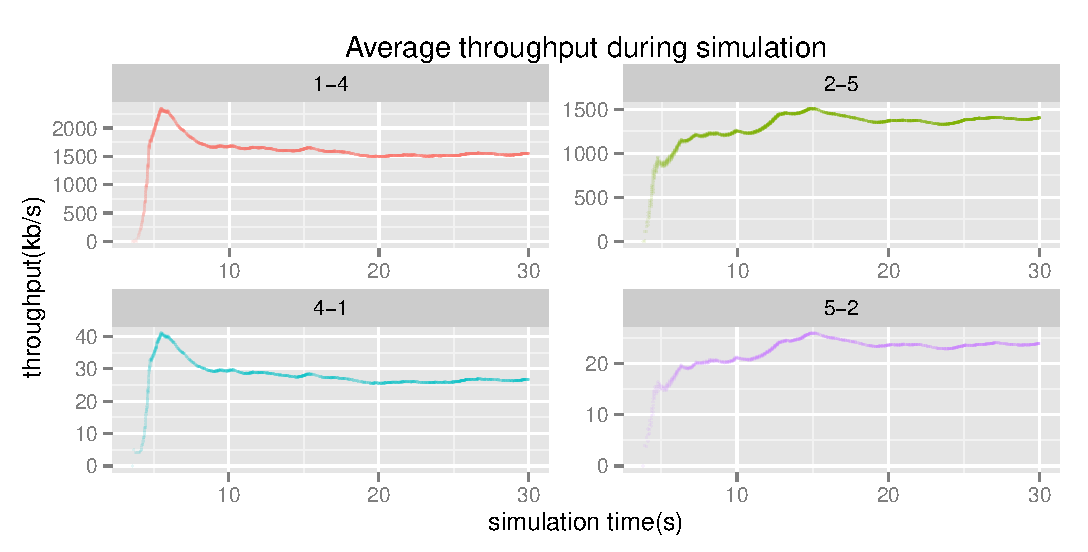
\includegraphics[width=1.02\textwidth]{pic/plot_cmt1_th_1.pdf}
	\end{figure}
\end{frame}

\begin{frame}
	\frametitle{\textbf{实验}2: \textbf{时延}}
	\begin{figure}
		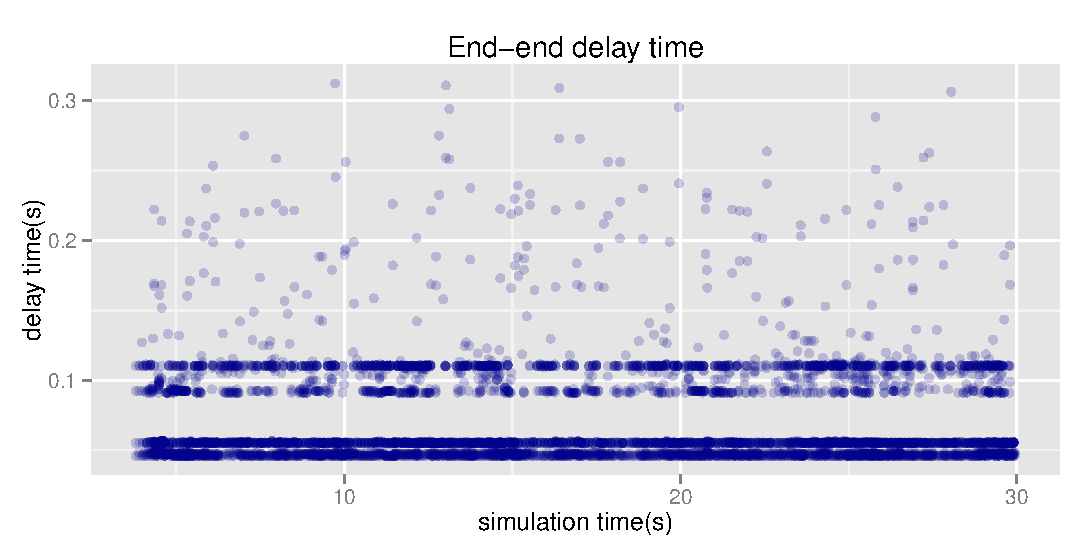
\includegraphics[width=\textwidth]{pic/plot_cmt1_delay_1.pdf}
	\end{figure}
\end{frame}

\begin{frame}
	\frametitle{\textbf{实验}2: cwnd}
	\begin{figure}
		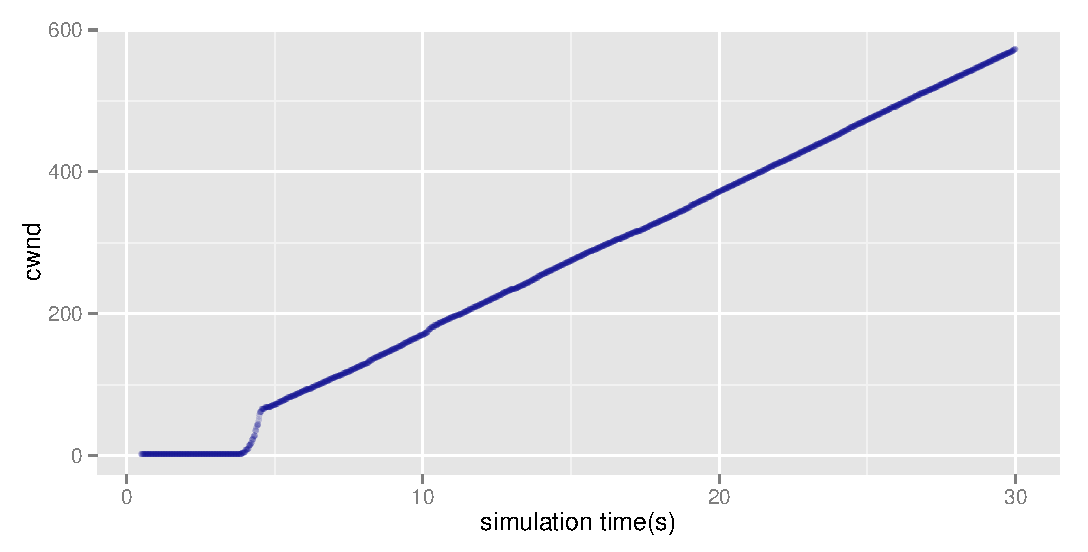
\includegraphics[width=0.9\textwidth]{pic/plot_cmt1_cwnd_1.pdf}
	\end{figure}
\end{frame}

\begin{frame}
	\frametitle{\textbf{实验}3}
	\framesubtitle{CMT\textbf{双向平行链路同带宽}}
		\begin{columns}
			\column{0.45\textwidth}
			\begin{picture}(100,40)(-30,0)
			
			
			\put(10,20){\circle{20}}
			\put(90,20){\circle{20}}
			\put(10,10){\line(1,0){80}}
			\put(10,30){\line(1,0){80}}
			\thicklines
			{\color{red}{\put(25,5){\vector(1,0){50}}}}
			{\color{red}{\put(25,35){\vector(1,0){50}}}}
			{\color{red}{\put(75,5){\vector(-1,0){50}}}}
			{\color{red}{\put(75,35){\vector(-1,0){50}}}}
			\thinlines
			\put(-35,16){{\footnotesize host\_0}}
			\put(105,16){{\footnotesize host\_1}}
			\put(-2,0){{\footnotesize if\_1\textcolor{blue}{{\itshape{(2)}}}}}
			\put(80,0){{\footnotesize if\_1\textcolor{blue}{{\itshape{(5)}}}}}
			\put(-2,32){{\footnotesize if\_0\textcolor{blue}{{\itshape{(1)}}}}}
			\put(80,32){{\footnotesize if\_0\textcolor{blue}{{\itshape{(4)}}}}}
			\end{picture}
			
			
			\column{0.5\textwidth}
			\begin{tabular}{c|c}
				\hline
				参数 & 值 \\
				\hline
				应用层 & FTP \\
				主地址 & if\_0(4) \\
				带宽(1-4) & 10Mb \\
				时延(1-4) & 45ms \\
				带宽(2-5) & 10Mb \\
				时延(2-5) & 45ms \\
				MTU & 1500 \\
				数据组块大小 & 1468 \\
				\hline
			\end{tabular}
		\end{columns}
\end{frame}

\begin{frame}
	\frametitle{\textbf{实验}3:\textbf{吞吐量}}
	\begin{figure}
		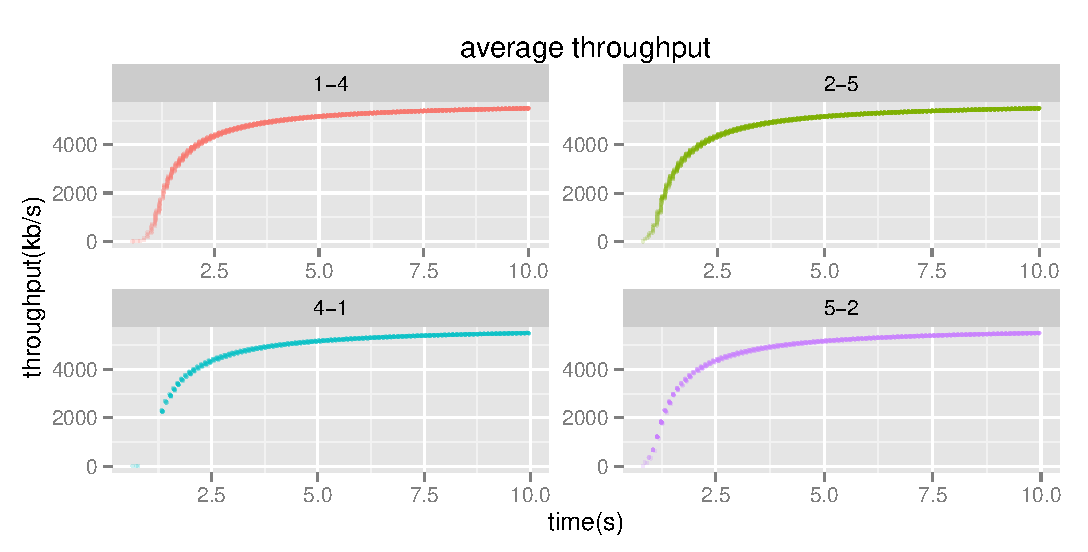
\includegraphics[width=\textwidth]{pic/plot_cmt2_th_1.pdf}
	\end{figure}
\end{frame}

\begin{frame}
	\frametitle{\textbf{实验}3:\textbf{时延}}
	\begin{figure}
		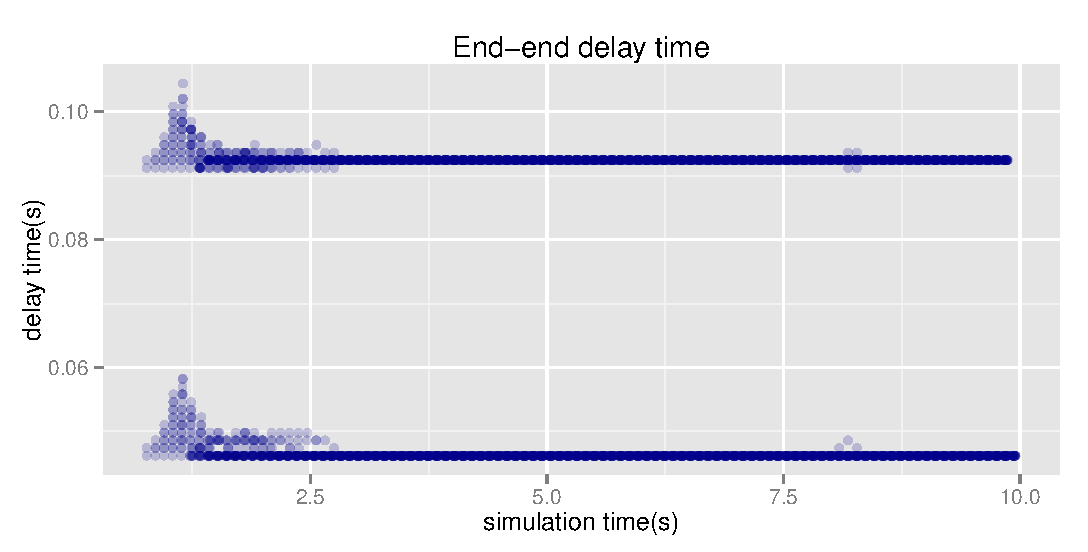
\includegraphics[width=\textwidth]{pic/plot_cmt2_delay.pdf}
	\end{figure}
\end{frame}

\begin{frame}
	\frametitle{\textbf{实验}4}
	\framesubtitle{\textbf{通过路由连接,使用心跳,中途更换主地址}}
	\begin{columns}
		\column{.45\textwidth}
		\begin{picture}(170,60)(-10,0)
			\put(25,30){\circle{30}}
			\put(155,30){\circle{30}}
			\put(90,30) {\circle{20}}
			\put(25,46) {\line(4,-1){55}}
			\put(25,14) {\line(4,1){55}}
			\put(155,46) {\line(-4,-1){55}}
			\put(155,14) {\line(-4,1){55}}
			\put(80,10) {\footnotesize router{\textcolor{blue}{\itshape(6)}}}
		    \put(10,6) {\footnotesize if\_0{\textcolor{blue}{\itshape(1)}}}
		    \put(140,6) {\footnotesize if\_0{\textcolor{blue}{\itshape(4)}}}
		    \put(10,47) {\footnotesize if\_1{\textcolor{blue}{\itshape(2)}}}
		    \put(140,47) {\footnotesize if\_1{\textcolor{blue}{\itshape(5)}}}
		    \put(-20,25){{\footnotesize host\_0}}
		    \put(172,25){{\footnotesize host\_1}}
		    \thicklines
		    {\color{red}{\put(40,14){\vector(4,1){30}}}}
		    {\color{red}{\put(40,46){\vector(4,-1){30}}}}
		    {\color{red}{\put(105,22){\vector(4,-1){30}}}}
		    {\color{red}{\put(102,40){\vector(4,1){30}}}}
		    \thinlines
		\end{picture}
		\\{\scriptsize *主地址在第7.5s时更换为if\_1(5)}
		\column{.5\textwidth}
		\begin{center}
		\begin{tabular}{c|c}
			\hline
			参数 & 值 \\
			\hline
			应用层 & FTP \\
			*主地址 & if\_0(4) \\
			带宽 & 0.5Mb \\
			时延 & 200ms \\
			MTU & 1500 \\
			数据组块大小 & 1468 \\
			\hline		
		\end{tabular}
		\end{center}
	\end{columns}
\end{frame}

\begin{frame}
	\frametitle{\textbf{实验}4:\textbf{吞吐量}}
	\begin{figure}
		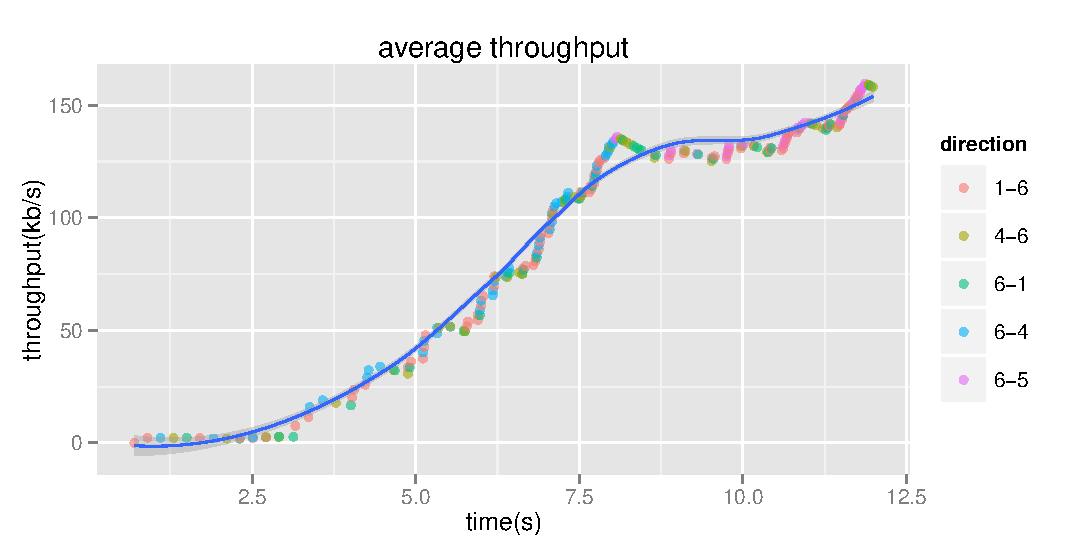
\includegraphics[width=1.05\textwidth]{pic/plot_router_th_1.pdf}
	\end{figure}
\end{frame}

\begin{frame}
	\frametitle{\textbf{实验}4:\textbf{吞吐量}}
		\begin{figure}
			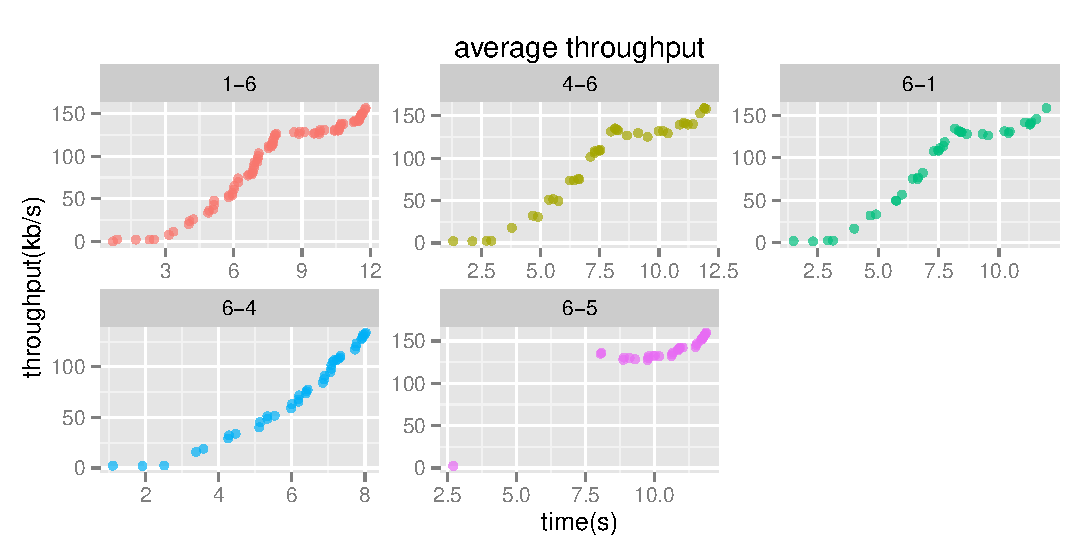
\includegraphics[width=1.05\textwidth]{pic/plot_router_th_2.pdf}
		\end{figure}
\end{frame}

\begin{frame}
	\frametitle{\textbf{实验}4:\textbf{封包}}
	\begin{figure}
		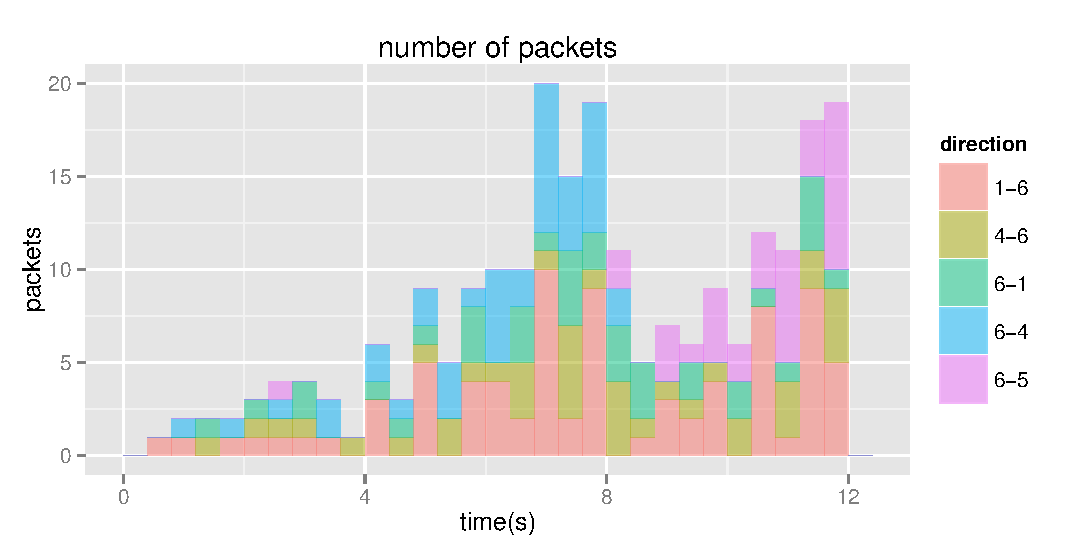
\includegraphics[width=1.05\textwidth]{pic/plot_router_fre.pdf}
	\end{figure}
\end{frame}

\begin{frame}
	\frametitle{\textbf{实验}4:\textbf{时延}}
	\begin{figure}
		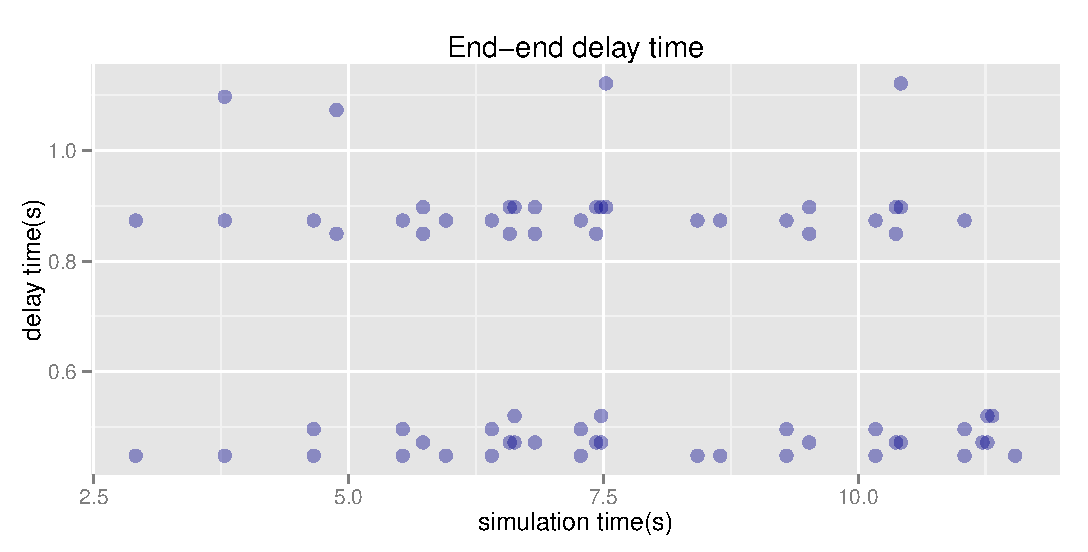
\includegraphics[width=\textwidth]{pic/plot_router_delay.pdf}
	\end{figure}
\end{frame}

\begin{frame}
	\frametitle{\textbf{实验}4:cwnd}
	\begin{figure}
		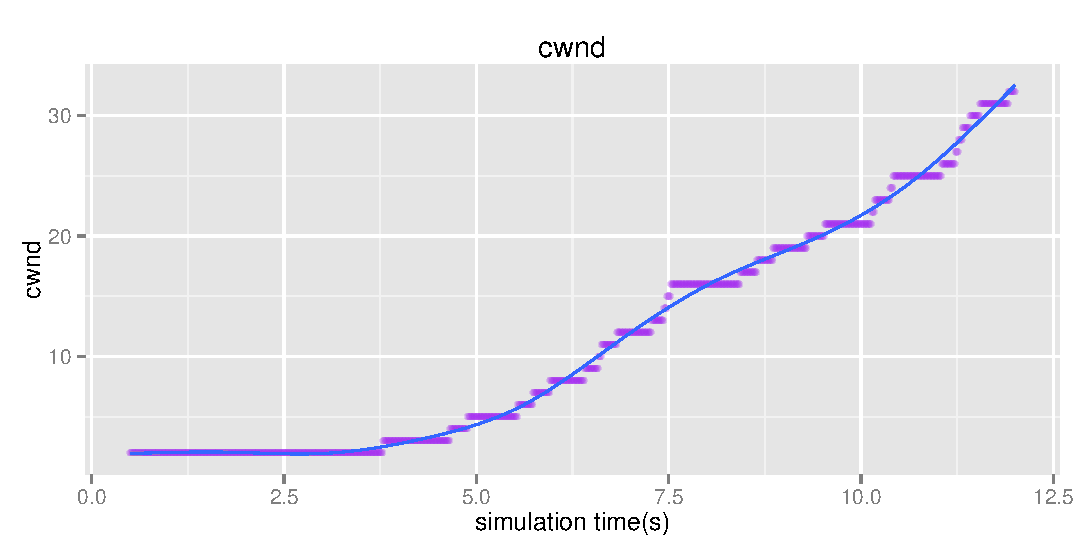
\includegraphics[width=\textwidth]{pic/plot_router_cwnd.pdf}
	\end{figure}
\end{frame}

\section{参考文献}
\begin{frame}
\frametitle{\textbf{参考文献}}
\bibliography{references}
\end{frame}

\section{结束语}
\begin{frame}
	\Huge{\centerline{The End}}
\end{frame}
%------------------------------------------------

%----------------------------------------------------------------------------------------

\end{document} 